\begin{frame}
    \frametitle{Cámara - Modelo Pin-Hole}
    
    \note{Ver libro de Sigwart. Seccion 4.2.3.2}
    \note{material sacado de mi tesis}
    
    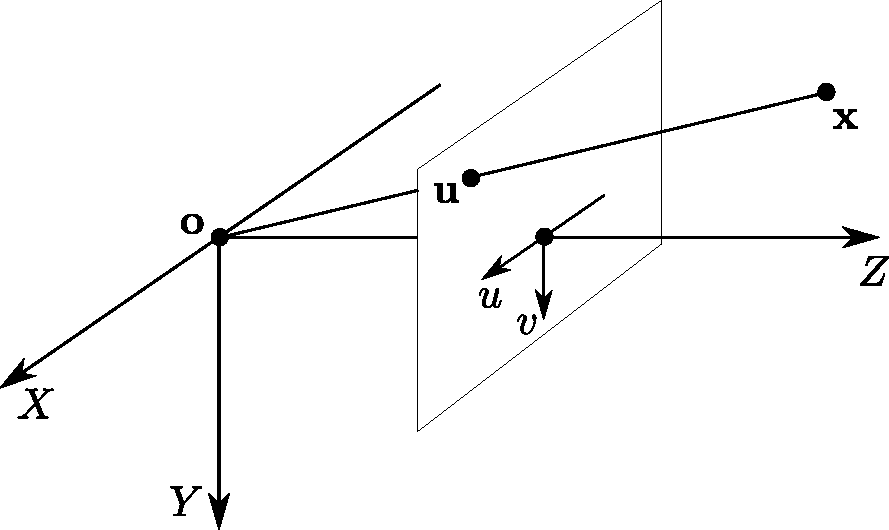
\includegraphics[width=0.4\columnwidth]{images/camera/pinhole_camera_model.pdf}
    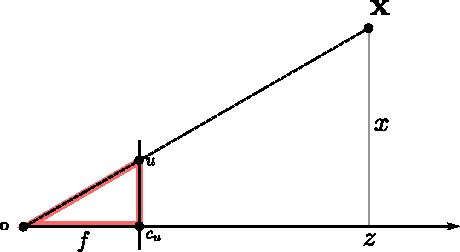
\includegraphics[width=0.4\columnwidth]{images/camera/pinhole_camera_model2.pdf}
    \footnotesize
    
    \begin{block}{Principio de funcionamiento}
    	En el modelo de cámara pinhole, el punto de la imagen $\imagePoint=\begin{bmatrix}u & v\end{bmatrix}^{\top}$ se determina como la intersección entre el plano de la imagen y el rayo que une el punto del mundo $\point =\begin{bmatrix}x & y & z\end{bmatrix}^{\top}$ y el centro de proyección $\cameraCenter$.
    \end{block}
  
    Denotamos con $\homo{\point}=\begin{bmatrix}x & y & z & 1\end{bmatrix}^{\top}$ la representación homogénea de un punto $\point=\begin{bmatrix}x & y & z\end{bmatrix}^{\top}$. Ahora, definimos el modelo de cámara:
    \begin{equation*}
        \imagePoint=f\proj(\cameraPoint)+\principalPoint
    \end{equation*}

    donde $f$ es la distancia focal, $\principalPoint$ es el punto principal, $\cameraPoint$ es el punto en el sistema de coordenadas de la cámara y la función $\proj:\mathbb{R}^{n}\rightarrow\mathbb{R}^{n- 1}$ se puede usar para transformar puntos de coordenadas homogéneas a no homogéneas, y también se puede usar para proyectar puntos del espacio 3D al plano de imagen 2D.
    \begin{equation*}
        \proj(\vec{a})=
            \frac{1}{a_{n}}\begin{bmatrix}a_{1}\\
            \vdots\\
            a_{n-1}
        \end{bmatrix}.
    \end{equation*}

    Por ejemplo, si $\point=\begin{bmatrix}x & y & z\end{bmatrix}^{\top}$, entonces $\proj(\point)=\begin{bmatrix}x/z & y/z\end{bmatrix}$.
    
    Se puede ver que $x/z=u/f$. Análogamente podemos decir que $y/z=v/f$. De estas ecuaciones podemos ver que $u=f(x/z)$ y que $v=f(y/z)$, por lo que la ecuación [eq:proyección] se cumple.
    
\end{frame}

\begin{frame}
    \frametitle{Cámara - Modelo Pin-Hole}
    
    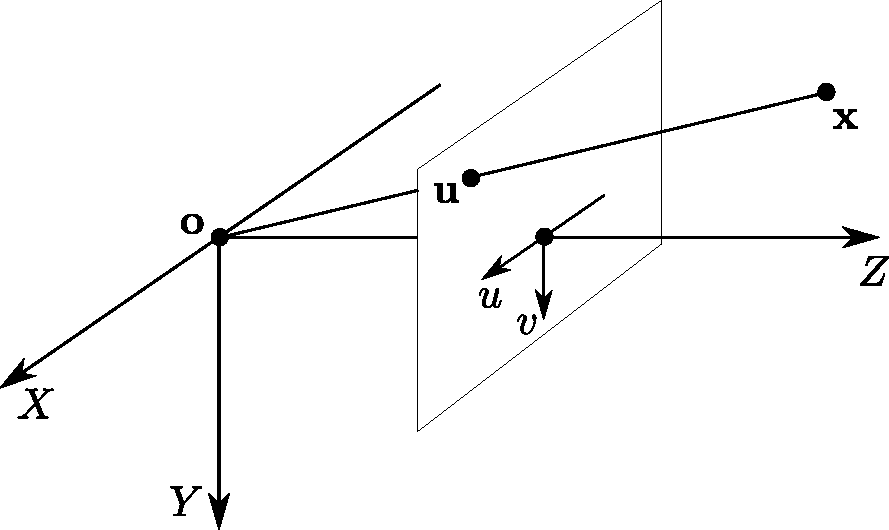
\includegraphics[width=0.4\columnwidth]{images/camera/pinhole_camera_model.pdf}
    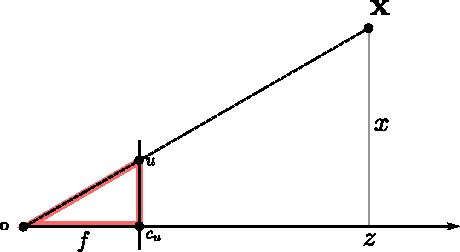
\includegraphics[width=0.4\columnwidth]{images/camera/pinhole_camera_model2.pdf}
    \footnotesize
    
    \begin{equation*}
        \proj(\vec{a})=
        \frac{1}{a_{n}}\begin{bmatrix}a_{1}\\
            \vdots\\
            a_{n-1}
        \end{bmatrix}.
    \end{equation*}
    
    Por ejemplo, si $\point=\begin{bmatrix}x & y & z\end{bmatrix}^{\top}$, entonces $\proj(\point)=\begin{bmatrix}x/z & y/z\end{bmatrix}$.
    
    Se puede ver que $x/z=u/f$. Análogamente podemos decir que $y/z=v/f$. De estas ecuaciones podemos ver que $u=f(x/z)$ y que $v=f(y/z)$, por lo que la ecuación [eq:proyección] se cumple.
    
\end{frame}


\begin{frame}
    \frametitle{Cámara - Modelo Pin-Hole}
    
    \footnotesize
    
    En el caso general, la cámara no está ubicada en el centro del sistema de coordenadas del mundo. Tenemos que agregar esta transformación entre el mundo y los sistemas de coordenadas de la cámara a la ecuación anterior, lo que da como resultado
    
    \begin{equation*}
        \imagePoint=f\proj(\proj(\seMatrix^{\mathrm{c}\mathrm{w}}\homoWorldPoint))+\principalPoint,
    \end{equation*}

    donde $\seMatrix^{\mathrm{c}\mathrm{w}}$ es una matriz de transformación que transforma elementos geométricos del marco de coordenadas del mundo $\mathrm{W}$ al marco de coordenadas de la cámara $\mathrm{C}$. Esto es,
    \begin{equation*}
        \homoCameraPoint=\seMatrix^{\mathrm{c}\mathrm{w}}\homoWorldPoint.
    \end{equation*}
   
\end{frame}

\begin{frame}
    \frametitle{Cámara - Modelo Pin-Hole}
    
    \footnotesize

    En particular, $\seMatrix^{\mathrm{c}\mathrm{w}}$ es una transformación que pertenece al Lie Group SE(3), el grupo de movimientos de cuerpo rígido en el espacio 3D. Por lo tanto, $\seMatrix^{\mathrm{c}\mathrm{w}}$ se define como
    $\seMatrix^{\mathrm{c}\mathrm{w}}=
    \begin{bmatrix}\rotation & \translation\\
        \vec{0} & 1
    \end{bmatrix}$ donde $\rotation$ es una matriz de rotación y $\translation$ es un vector de traslación. Observe que una de las ventajas de trabajar con coordenadas homogéneas es que permite utilizar el álgebra de Grupos de Lie SE(3).
    
    Existe una notación de matriz para el modelo de cámara pin-hole que también se usa comúnmente en visión por computadora.
    \begin{equation*}
        \projectionMatrix=\intrinsicMatrix\begin{bmatrix}\rotation & \translation\end{bmatrix}
    \end{equation*}

    donde $\projectionMatrix$ es la matriz de proyección y $\intrinsicMatrix$ es la matriz de calibración. La matriz de calibración se define como,
    
    \begin{equation*}
        \intrinsicMatrix=
        \begin{bmatrix}f & 0 & c_{u}\\
            0 & f & c_{v}\\
            0 & 0 & 1
        \end{bmatrix},
    \end{equation*}

\end{frame}

\begin{frame}
    \frametitle{Cámara - Modelo Pin-Hole}
    
    \footnotesize

    Siendo $\begin{bmatrix}c_{u} & c_{v}\end{bmatrix}^{\top}$ la posición del punto principal. Entonces, usando la matriz de proyección $\projectionMatrix$, el punto del mundo $\worldPoint$ se asigna al punto imagen $\imagePoint$ por
    \begin{equation*}
    \imagePoint=\proj{(\projectionMatrix\homoWorldPoint)}.
    \end{equation*}

\end{frame}


\begin{frame}
	\frametitle{Distorción}
    
    Previamente, consideramos que el modelo de cámara pin-hole es perfectamente lineal, es decir, el punto en el mundo, el punto en la imagen y el centro óptico son colineales.
	
    Esta suposición no es cierta en la práctica porque hay una distorsión radial en la imagen producida por la lente de la cámara real. La figura presenta algunas distorsiones comunes generadas por la lente.
    
    
    
   	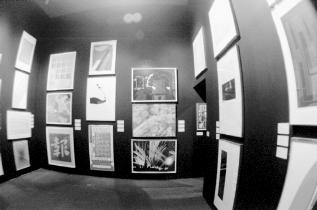
\includegraphics[width=0.4\columnwidth]{images/camera/distorted_image.png}
    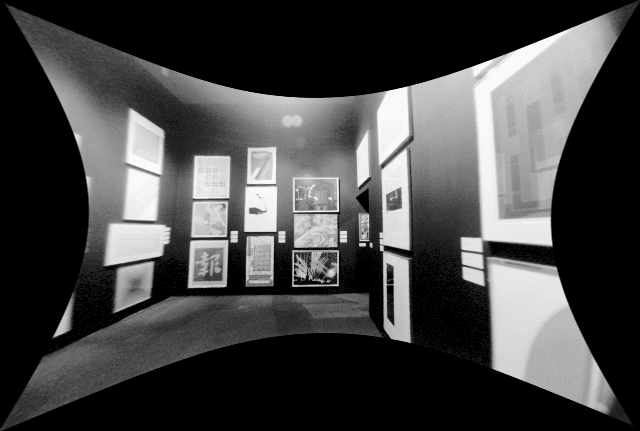
\includegraphics[width=0.4\columnwidth]{images/camera/undistorted_image.png}
	
\end{frame}


\begin{frame}
    \frametitle{Distorción}
    
    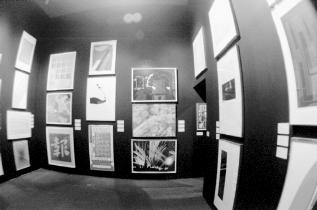
\includegraphics[width=0.4\columnwidth]{images/camera/distorted_image.png}
    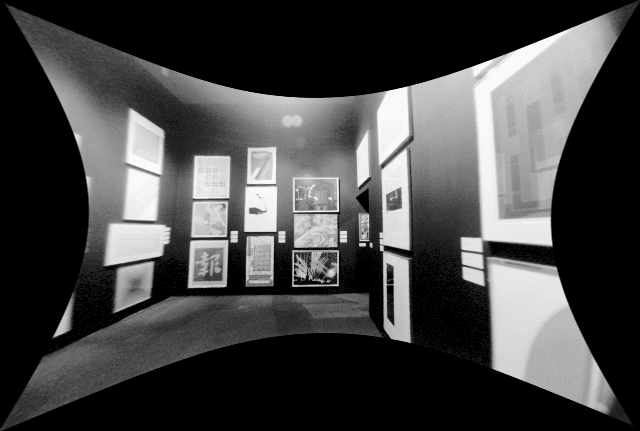
\includegraphics[width=0.4\columnwidth]{images/camera/undistorted_image.png}
    
\end{frame}


\begin{frame}
	\frametitle{Características Visuales: Detector FAST}
	
	\begin{figure}
		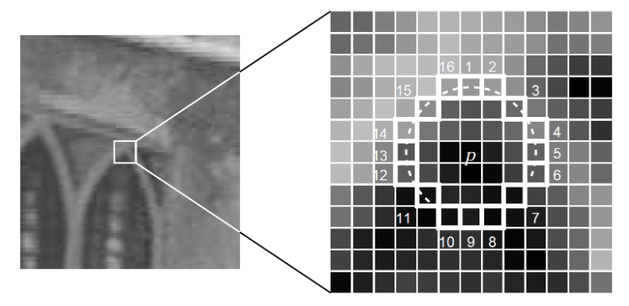
\includegraphics[width=0.8\textwidth]{./images/camera/fast}
	\end{figure}
	
	El valor de intensidad del pixel $p$ es comparado con cada uno de los 16 pixeles del círculo de Bresenham alrededor de $p$. $p$ es detectado como corner si hay $12$ píxeles continuos en el circulo de Bresenham más brillosos o oscuros que $p$ dado un cierto umbral.
\end{frame}

\begin{frame}
	\frametitle{Características Visuales: Descriptor BRIEF}
	\begin{minipage}[t]{0.35\columnwidth}
		\begin{figure}
			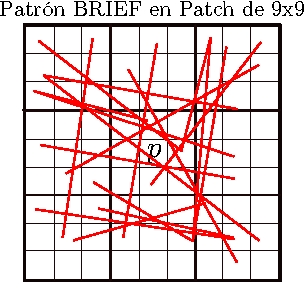
\includegraphics[width=\columnwidth]{./images/camera/brief}
		\end{figure}
	\end{minipage}\hfill{}
	\begin{minipage}[t]{0.6\columnwidth}
		\centering
		256 Comparaciones entre píxeles (1 a 1)
		\begin{equation*}
			\tau(p;x,y) =
			\begin{cases}
				1 & \text{if $p(x) < p(y)$}\\
				0 & \text{otherwise}\\
			\end{cases}     
		\end{equation*}
		$s = \overbrace{01010010101110010...}^{256\ \text{bits}}$
	\end{minipage}
	\begin{block}{Matching distance}
		$\text{Hamming distance} = sum (XOR(s_{1}, s_{2}))$
	\end{block}
	\note{utilizamos la distancia de hamming para la distancia de matcheo entre descriptores.}
\end{frame}
